\documentclass[a4paper,10.9pt]{article}

% Packages
\usepackage[utf8]{inputenc}
\usepackage[T1]{fontenc}
\usepackage[french]{babel}
\usepackage{amsmath,amsfonts,amssymb}
\usepackage{amsthm}
\usepackage{graphicx}
\usepackage[a4paper, margin=1cm]{geometry}
\usepackage{fancyhdr}
\usepackage{lastpage}
\usepackage{lipsum} % Pour générer du faux texte. À retirer dans le document final.
\usepackage{cite}
\usepackage{hyperref}
\usepackage{url}

% Paramètres de la page
\geometry{top=2.5cm, bottom=2.5cm, left=2.2cm, right=2.2cm}
\pagestyle{fancy}
\fancyhf{}
\rhead{Caucheteux Maxence}
\lhead{Parcours Recherche}
\rfoot{Page \thepage/\pageref{LastPage}}
\renewcommand{\headrulewidth}{2pt}
\renewcommand{\footrulewidth}{1pt}
\setlength{\parindent}{0pt}


% Titre du document
\title{Parcours Recherche}
\author{Maxence Caucheteux}
\date{\today}

% Macros
\newcommand{\E}{\mathbb{E}}
\newcommand{\prob}{\mathbb{P}}
\newcommand{\R}{\mathfrak{R}_0}


\begin{document}

\maketitle

\vspace{1em}
\vspace{1em}
\vspace{1em}

\begin{center}
    \textsc{\LARGE Ecole Nationale des Ponts et Chaussées}
\end{center}

\vspace{1em}

\begin{figure}[h]
    \centering
    \includegraphics[width=150px, height=200px]{logo_ponts_0.png}
\end{figure}

\setlength{\arrayrulewidth}{2pt}

\vspace{1em}

\rule{\textwidth}{2pt}

\vspace{1em}

\begin{center}
    \textsc{\LARGE Épidémiologie et Déplacements}
\end{center}

\rule{\textwidth}{2pt}


\vspace{4em}
\begin{center}
	{\Large Ce projet a été effectué sous la supervision de }\\
	\vspace{0.3cm}
	{\huge Jean-François DELMAS}
\end{center}

\newpage

\tableofcontents

\newpage

\textbf{ABSTRACT :} This article investigates the role of individual mobility in shaping epidemic dynamics within the susceptible-infectious-susceptible (SIS) model framework. Beginning with an exploration of epidemiology and associated mathematical models, we introduce a stochastic model formulated using Markov chains to capture epidemic spread dynamics. Transitioning to a deterministic model by scaling as the size of the population goes to infinity, we establish relationships between model parameters, particularly focusing on fundamental epidemic metrics such as the basic reproduction number $\R$. Through analysis of the resulting deterministic equations, we examine how varying degrees of individual mobility influence epidemic progression.

\section{Introduction}
On s'intéresse à un modèle d'épidémie élémentaire, à savoir le modèle susceptible-infecté-susceptible (SIS). Dans ce modèle, les individus sont soit susceptibles, soit infectés. On dit que c'est un \textbf{modèle compartimental} (voir \cite{CompartmentalModels}). Les individus infectés peuvent guérir et les individus susceptibles peuvent s'infecter. Dans ce projet, on considère une population répartie dans différentes villes. Les individus peuvent passer d'une ville à l'autre via des déménagements.\\

\textbf{Le but du projet est d'étudier l'impact du
déplacement des individus sur la propagation de l'épidémie.} \\

Plus précisément : \\
-- On se familiarise d'abord avec l'épidémiologie et aux modèles mathématiques associés. \\
-- On propose un modèle stochastique modélisant une épidémie à l'aide de chaînes de Markov. \\
-- On essaie de construire un modèle déterministe à partir du modèle stochastique par passage à la limite et on regarde dans quelle mesure les deux modèles correspondent.  \\
-- On définit les grandeurs naturelles (nombre de reproduction de base $\R$...) sur le modèle déterministe et on fait le lien entre les paramètres des deux modèles. \\
-- On étudie les équations déterministes obtenues par passage à la limite. \\
-- On regarde finalement comment évolue l'épidémie selon qu'on laisse plus ou moins les individus se déplacer librement.

\newpage

\section{Modèle à un compartiment}

\subsection{Construction du modèle}
Étudions dans un premier temps un modèle simplifié de population homogène. \\

On fait évoluer l'épidémie selon le processus suivant. On choisit un individu parmi les $N$ individus :

-- Si cet individu est infecté, il guérit avec probabilité $p$.

-- S'il est susceptible, il devient infecté avec probabilité $q \times \tau$ où $\tau$ est la proportion d'infectés. \\

Selon ce processus on construit des chaînes de Markov.

On définit un système dynamique stochastique $(\mathcal{I}_t^N)$, qui modélise les personnes infectées de la population. Le processus $(\mathcal{I}_t^N)$ est à valeur dans $\{0,1\}^N$ : les coefficients sont égaux à $1$ pour les personnes infectées et les autres coefficients sont nuls pour les personnes susceptibles. \\

On se donne différentes variables aléatoires :

-- Soit $(X_t)_{t \in \mathbb{N}^*}$ une suite de variables aléatoires indépendantes identiquement distribuées (VAIID) suivant la loi uniforme $\mathcal{U}([1,N])$. Ces variables vont nous permettre de modéliser le choix d'une personne dans la population à chaque instant discret.

-- Soit $(B^g_t)_{t \in \mathbb{N}^*}$ une suite de VAIID suivant la loi de Bernoulli $\mathcal{B}(p)$. Ces variables vont nous permettre de dire si la personne guérit si elle est infectée.

-- Pour $k \in [0,N]$ soit $(B^i_{\tau(k),t})_{t \in \mathbb{N}^*}$ une suite de VAIID suivant la loi de Bernoulli $\mathcal{B}(q \tau(k))$ où $\tau(k)=\frac{k}{N}$ est appelé \textbf{taux d'infection d'ordre $k$}. On appelle également $T=\{\tau(k) \ | \ k \in [0,N]\}$ l'ensemble de ces taux. Les variables précédentes vont nous permettre de dire s'il y a infection si la personne choisie est saine. \\

On suppose que les suites de variables aléatoires introduites ci-dessus sont indépendantes et on se donne $\mathcal{I}_0$ une variable aléatoire à valeur dans $\{0,1\}^N$ indépendante de toutes les précedentes et qu'on pourra choisir déterministe. \\

On peut alors construire $\mathcal{I}^N=(\mathcal{I}^N_t)_{t \geq 0}$ en posant $\mathcal{I}^N_0=\mathcal{I}_0$ et pour $t \geq 0$,
$$\boxed{ \mathcal{I}_{t+1}^N = \left\{
\begin{array}{ll}
        \mathcal{I}_t^N-B_{t+1}^g e_{X_{t+1}} \ \ \operatorname{si} \mathcal{I}^N_{t,X^1_t}=1 \\
        \mathcal{I}_t^N+B_{\tau \left(\sum_{k=1}^N \mathcal{I}_{t,k}^N \right),t+1}^i e_{X_{t+1}} \ \ \operatorname{sinon}
\end{array}
\right. }$$
où $(e_k)$ est la base canonique de $\mathbb{R}^N$. Cette définition de $\mathcal{I}^N$ traduit bien le processus intuitif défini précédemment. \\

En posant $V_{t+1}=(X_{t+1}, B^g_{t+1}, (B_{\tau, t+1})^i_{\tau \in T})$, on peut écrire :
$$\boxed{\mathcal{I}_{t+1}^N = f(\mathcal{I}_t^N, V_{t+1})}$$
avec pour $g \in \{0,1\}^N$, $k \in [1,N]$, $m \in \{0,1\}$ et $(m_{\tau})_{\tau \in T} \in \{0,1\}^T$ :
$$\boxed{ f(g,k,m,(m_{\tau})_{\tau \in T}) = \left\{
\begin{array}{ll}
        g-m e_k \ \ \operatorname{si} \ g_k=1  \\
        g + m_{\tau\left(\sum_{p=1}^N g_p\right)}e_k \ \ \operatorname{si} \ g_k=0
\end{array}
\right. }$$
Ainsi, $\mathcal{I}^N$ est un \textbf{système dynamique stochastique} donc une chaîne de Markov (voir \cite{DelmasCourse}, chapitre 3). \\

\subsection{Propriétés : matrices de transition}

On note $P$ la matrice de transition de $\mathcal{I}^N$. Il s'agit d'une matrice carrée de taille $2^N$. On a le résultat suivant : \\

\begin{tabular}{|c}
\begin{minipage}{\textwidth}
\textbf{Proposition}

Pour $x,y \in \{0,1\}^N$, en notant $I=\sum_{k=1}^N x_k$ le nombre de personnes infectées et $|.|$ la norme $1$, on a :
\[\boxed{
P(x,y) = \left\{
\begin{array}{ll}
0 & \text{si } |x-y| > 1 \\
\frac{p}{N} & \text{si } y=x-e_i \\
\frac{q I}{N^2} & \text{si } y=x+e_i
\end{array}
\right. }
\]
Comme $P$ est stochastique, on peut utiliser ce qui précède pour calculer $P(x,x)$ via la formule :
$$P(x,x)=1-\sum_{y \neq x} P(x,y)$$
\end{minipage}
\end{tabular} \\

On remarque que l'état $(0,...,0)\in \{0,1\}^N$ est \textbf{absorbant}. Par ailleurs, depuis chaque état, on va à l'état $(0,...,0)$ avec probabilité non nulle. Par suite, tous les états, excepté $(0,...,0)$ sont \textbf{transients}. Comme une mesure invariante ne charge pas les états transients (voir \cite{DelmasCourse}), on en déduit que $P$ admet une unique mesure invariante qui est $\pi_1(x)=0$ si $x \neq (0,...,0)$ et $1$ sinon. Cela signifie qu'à l'équilibre la maladie a disparu. \\

On définit le nombre d'infectés à l'instant $t$ par $I^N_t=\sum_{k=1}^N \mathcal{I}_{t,k}^N$.  \\

En général, l'image d'une chaîne de Markov par une application n'est pas une chaîne de Markov. Cependant, c'est vrai ici par \textbf{lemme de la chaîne image} (par l'application $\varphi : \{0,1\}^N \longrightarrow [0,N], x \mapsto \sum_{k=1}^N x_k$), dont on trouve l'énoncé ainsi qu'une démonstration dans \cite{HenardExercises} : \\

\begin{tabular}{|c}
\begin{minipage}{\textwidth}
\textbf{Proposition}

Pour $k \in [0,N]$,
$$\boxed{\left\{
\begin{array}{ll}
        Q(k,k-1)=p\frac{k}{N} \ \ \operatorname{si} k \geq 1 \\
        Q(k,k+1)=q\frac{k}{N} (1-\frac{k}{N}) \ \ \operatorname{si} \ k<N \\
        Q(k,k)=(1-\frac{k}{N})(1-\frac{k}{N}q)+\frac{k}{N}(1-p)
\end{array}
\right. }$$
Les autres coefficients de la matrice $Q$ sont nuls. \\

De plus, $\pi_2(k)=0$ si $k \neq 0$ et $1$ sinon est l'unique mesure invariante pour $Q$. 
\end{minipage}
\end{tabular} \\

On s'attendait à ce résultat car :

-- Pour passer de $k$ infectés à $k-1$ infectés, il faut qu'on choisisse un infecté, ce qui arrive avec probabilité $\frac{k}{N}$, et que celui-ci guérisse, ce qui arrive avec probabilité $p$.

-- Pour passer de $k$ à $k+1$ infectés, il faut qu'on choisisse un individu sain, ce qui arrive avec probabilité $1-\frac{k}{N}$ et que celui-ci tombe malade, ce qui arrive avec probabilité $q\tau=q\frac{k}{N}$.

-- L'expression de $Q(k,k)$ est issue d'une ré-écriture puisque $Q(k,k)=1-Q(k,k-1)-Q(k,k+1)$. Cette écriture est même vraie lorsque $k$ vaut une des bornes de $[0,N]$. 

-- Les autres coefficients sont nuls car si on a $k$ infectés, par définition du processus, on peut soit garder le même nombre d'infectés $k$, soit le modifier d'une unité, en plus ou en moins et ainsi obtenir $k \pm 1$ infectés.  \\

L'expression de la mesure invariante de $Q$ traduit de nouveau l'idée qu'à l'équilibre la maladie a disparu. \\

On calcule en Python les coefficients de cette matrice dans quatre cas, avec les paramètres $N=6$, $q=0,9$ et on choisit quatre valeurs de $p$ différentes (figure~\ref{fig:trans}). \\

\begin{figure}[h!]
  \centering
  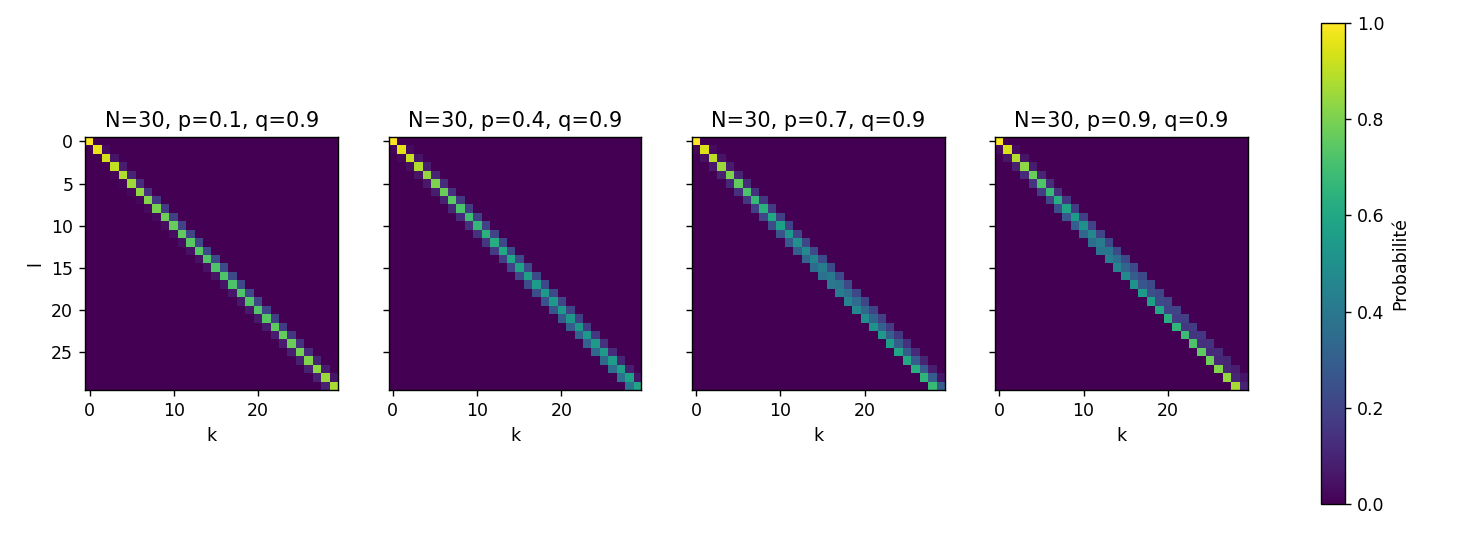
\includegraphics[width=0.6\textwidth]{im6-pr.png} % Ajustez le coefficient en fonction de vos besoins
  \caption{Matrice de transition de $I^N$ dans quatre cas}
  \label{fig:trans}
\end{figure}

\subsection{Modèle déterministe : SIS}
\subsubsection{Introduction du modèle}
Ce modèle déterministe, décrit dans \cite{sis} (chapitre $3$), permet de modéliser l'évolution du nombre d'individus susceptibles $S$ et infectés $I$ par des équations différentielles. Ce modèle est décrit par le système d'équations suivant : 
$$\left\{
\begin{array}{ll}
        \frac{dS}{dt}=-KSI+\gamma I \\
        \frac{dI}{dt}=KSI-\gamma I 
\end{array}
\right. $$
avec $I$ à valeurs positives. \\
$K$ et $\gamma$ sont deux constantes strictement positives. $K$ est appelé \textbf{taux de transmission} de la maladie et \textbf{$\gamma$ vitesse de guérison} de la maladie. \\

On constate de plus que le nombre de personnes $I+S=N$ est constant en sommant ces deux équations. On regarde plutôt le taux d'infectés $I/N$ et le taux de susceptibles $S/N$. Par abus, on note encore $I$ et $S$ ces taux. Ainsi, avec cet abus, $S=1-I$ et en injectant $S$ sous cette forme dans la deuxième équation ci-dessus on obtient :
$$\boxed{\frac{dI}{dt}=(1-I)KI-\gamma I}$$
On retrouve sur cette équation le sens biologique du modèle. Le terme $(1-I)KI$ est lié aux infections (choix d'un infecté avec probabilité $I$, d'un susceptible avec probabilité $1-I$ et on multiplie par le taux de transmission $K$) et le terme $\gamma I$ aux guérisons.

\subsubsection{Résolution}
On cherche les solutions de l'équation précédente à valeurs dans $]0,1]$. On a la résultat suivant : \\

\begin{tabular}{|c}
\begin{minipage}{\textwidth}
\textbf{Proposition}


On pose $\mathfrak{R}_0=\frac{K}{\gamma}$, appelé nombre de reproduction de base. Alors, pour $t \geq 0$,
$$ I(t)= \left\{
\begin{array}{ll}
          \frac{\mathfrak{R}_0-1}{\left(\frac{1}{I_0}(\mathfrak{R}_0-1)-\mathfrak{R}_0 \right)e^{-\gamma(\mathfrak{R}_0-1)t}+\mathfrak{R}_0} \ \ \operatorname{si} \mathfrak{R}_0 \neq 1 \\
          \frac{1}{\frac{1}{I_0}+\gamma t} \ \ \operatorname{si} \mathfrak{R}_0=1
\end{array}
\right. $$
où $I(0)=I_0 \in ]0,1]$ 
\end{minipage}
\end{tabular} \\

\begin{proof}
Pour justifier cette affirmation, on écrit l'équation sous la forme :
$$\frac{dI}{dt}=(K-\gamma)I-KI^2$$
Il s'agit d'une équation de Bernoulli. Pour la résoudre, on effectue le changement de variable $u(t)=\frac{1}{I(t)}$. On obtient alors une équation sur $u$ :
$$\frac{du}{dt}=(\gamma-K)u(t)+K$$
Il s'agit d'une équation différentielle linéaire d'ordre $1$ dont on connaît les solutions. On en déduit ainsi l'expression de $u(t)$ puis celle de $I(t)$. \\
\end{proof}

On remarque que :

\textbf{1/} Si $\mathfrak{R}_0>1$, on a : 
$$I(t)\mathop{\longrightarrow}_{t \rightarrow \infty}\frac{\mathfrak{R}_0-1}{\mathfrak{R}_0}>0$$
La maladie subsiste.

\textbf{2/} Si $\mathfrak{R}_0<1$, $I(t)$ tend vers $0$ en temps long et cette convergence est exponentielle.

\textbf{3/} Si $\mathfrak{R}_0=1$, $I(t)$ tend vers $0$ en temps long mais la convergence n'est pas exponentielle mais simplement en $\frac{1}{t}$. \\

Dans les deux derniers cas, la maladie disparaît. \\

En pratique, le calcul du $\R$ est difficile puisqu'il dépend de nombreux facteurs (régionaux, comportementaux, sociaux etc). Cependant, pour des maladies communes, le tableau suivant (issu de \cite{R0}) fournit une estimation du $\R$ :

\[
\begin{array}{|c|c|}
\hline
\textbf{Maladie} & \R \\
\hline
\text{Rougeole} & 12 - 18 \\
\text{Varicelle} & 10 - 12 \\
\text{Rubéole} & 6 - 7 \\
\text{COVID-19} & 2.5 - 3.5 \\
\text{Tuberculose} & 2 - 3 \\
\text{Rhume commun} & 2 - 3 \\
\text{Grippe} & 1.3 - 1.8 \\
\hline
\end{array}
\]

La figure~\ref{fig:taux_inf} montre comment évolue le taux d'infectés en partant d'une population initialement infectée à hauteur de $50$\% pour différentes valeurs de $\R$.

\begin{figure}[h!]
  \centering
  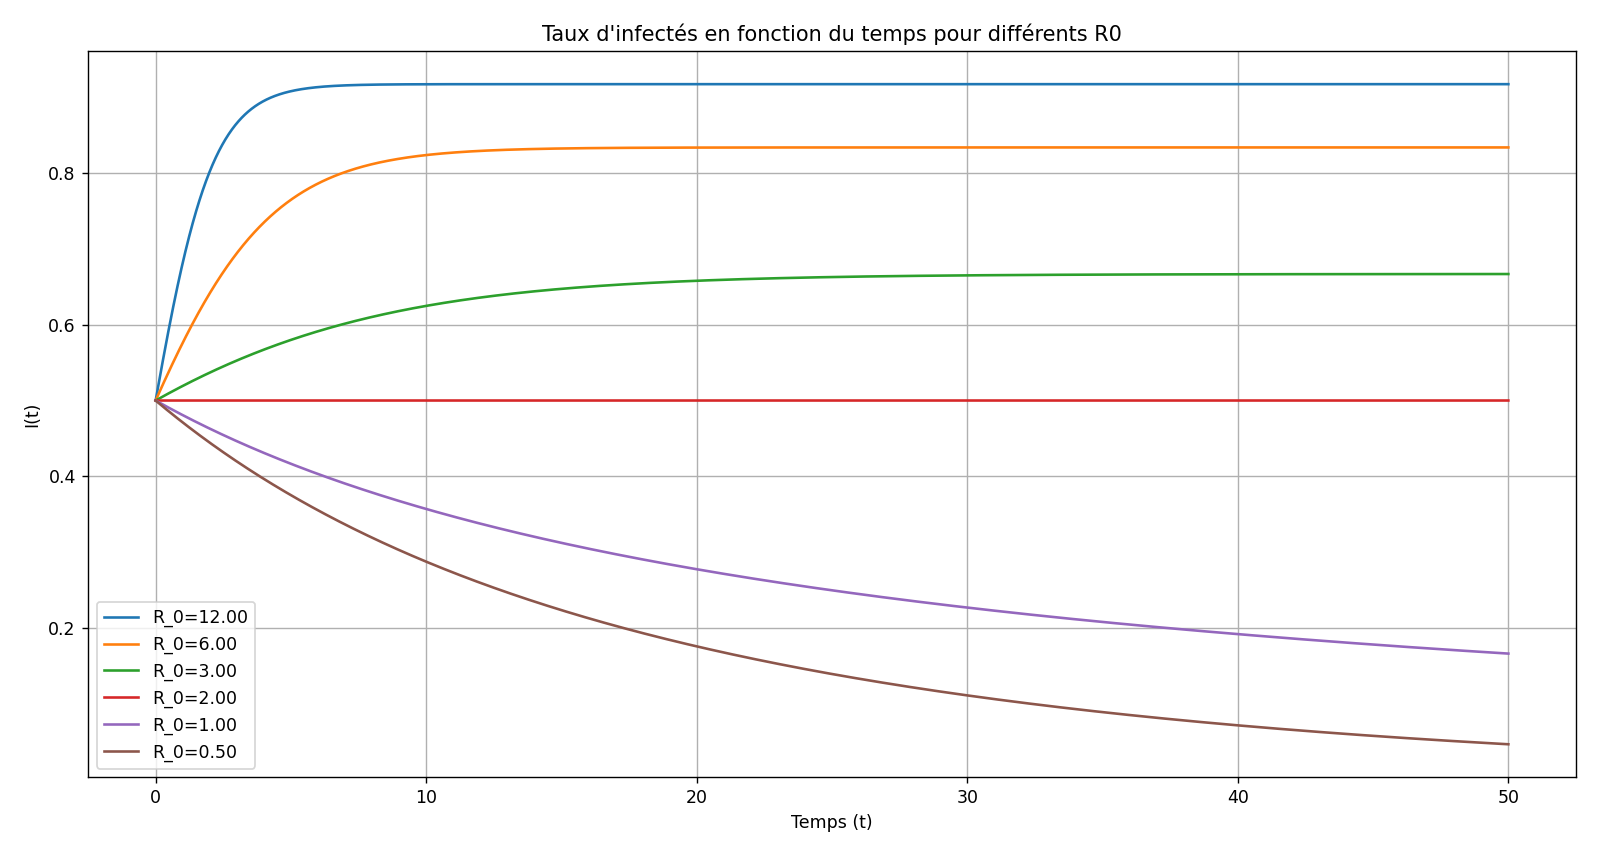
\includegraphics[width=0.7\textwidth]{im4-pr.png} % Ajustez le coefficient en fonction de vos besoins
  \caption{Évolution du taux d'infectés avec différents $\mathfrak{R}_0$}
  \label{fig:taux_inf}
\end{figure}

Le modèle SIS peut être étendu à plusieurs groupes en introduisant une \textbf{matrice de contact} $K$ entre les groupes. On a alors un système d'équations différentielles qu'il n'est pas possible de résoudre analytiquement. Cependant, Lajmanovich et Yorke \cite{LajmanovichYorke} ont réussi à montrer que le comportement des solutions en temps long dépend uniquement du nombre de reproduction de base.

\subsection{Lien entre le modèle SIS et le processus stochastique}
\subsubsection{Construction d'un modèle déterministe à partir du modèle stochastique}

On cherche à montrer un lien entre les paramètres du modèle SIS et ceux de la chaîne de Markov introduite précédemment. Ces deux modèles décrivent l'évolution d'une épidémie qui présente les mêmes caractéristiques : on est soit infecté, soit susceptible ; et les individus susceptibles peuvent devenir infectés ; et réciproquement les infectés peuvent guérir. C'est pourquoi nous sommes légitimes de vouloir faire ce lien. \\


Intuitivement, en regardant ce qu'il se passe à l'instant discret $t=1$, on veut pouvoir approcher $\frac{1}{N} I^N_1$ de $I(\Delta_N)$ en grandes populations (i.e. $N$ grand), où $(\Delta_N)$ est un pas de temps qui tend vers $0$. C'est pourquoi, afin d'obtenir par identification un lien entre les paramètres des deux modèles, on peut envisager l'approximation suivante :
$$\frac{1}{N}\mathbb{E}_k(I^N_1) \simeq I(\Delta_N)=I(0)+\Delta_N I'(0)+o(\Delta_N)=\frac{k}{N}+\Delta_N \left( \left(1-\frac{k}{N} \right)K\frac{k}{N}-\gamma \frac{k}{N} \right)+o(\Delta_N)$$
Un calcul montre que :
$$\frac{1}{N}\mathbb{E}_k(I^N_1)=\frac{k}{N}+\frac{1}{N} \left( \left(1-\frac{k}{N} \right)\frac{k}{N}q-p\frac{k}{N} \right)$$
On en déduit : 
$$\boxed{\Delta_N=\frac{1}{N}, \ \gamma=p \text{ et } K=q}$$

Le pas $\Delta_N=\frac{1}{N}$ montre que pour passer du temps continu au temps discret (et réciproquement), il faut utiliser l'échelle de temps :
$$t_{\text{discret}}=\lfloor Nt \rfloor$$

\subsubsection{Illustration par des simulations}
Simulons via Python l'évolution du nombre d'infectés avec le jeu de paramètres suivants : $N=300$ personnes dont $k=150$ personnes infectées initialement, $p=0,7$ et $q=0,3$ ($\mathfrak{R}_0<1$). On représente sur chaque graphe la courbe du nombre d'infectés en temps discret donné par l'équation déterministe du modèle SIS, noté $\tilde{I}_N$ et donné par :
$$\forall n, \ \tilde{I}_N(n)=N I_N(n/N)$$
où $I_N$ est la solution du modèle SIS décrit dans une section précédente, avec la condition initiale $I_N(0)=\frac{k}{N}$.
On effectue $3$ puis $40$ simulations (figure~\ref{fig:nb_inf1}).

\begin{figure}[h!]
  \centering
  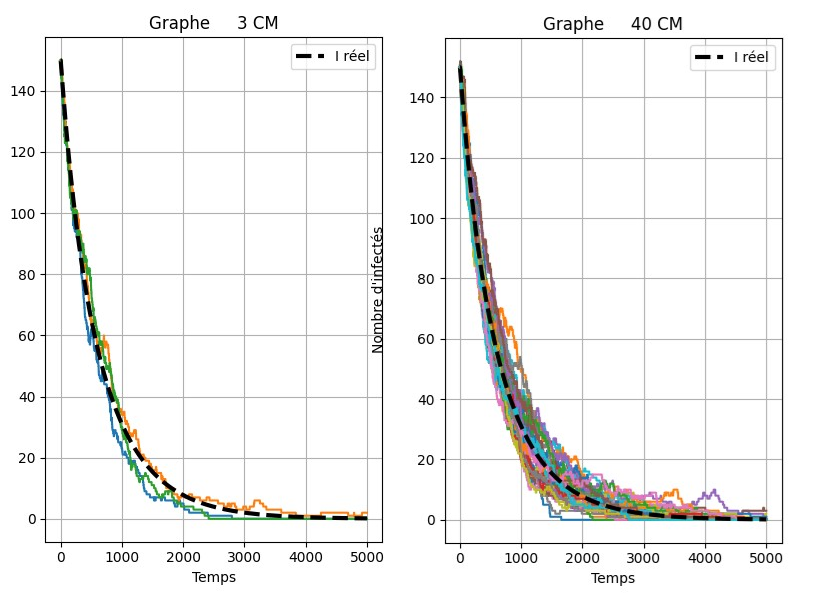
\includegraphics[width=0.45\textwidth]{im8-pr.png} % Ajustez le coefficient en fonction de vos besoins
  \caption{Évolution du nombre d'infectés}
  \label{fig:nb_inf1}
\end{figure}

On peut changer les valeurs de $p$ et $q$ afin que $\mathfrak{R}_0>1$. On part cette fois-ci de $100$ infectés. On effectue le même tracé avec $3$ puis $10$ simulations (figure~\ref{fig:nb_inf2}).

\begin{figure}[h!]
  \centering
  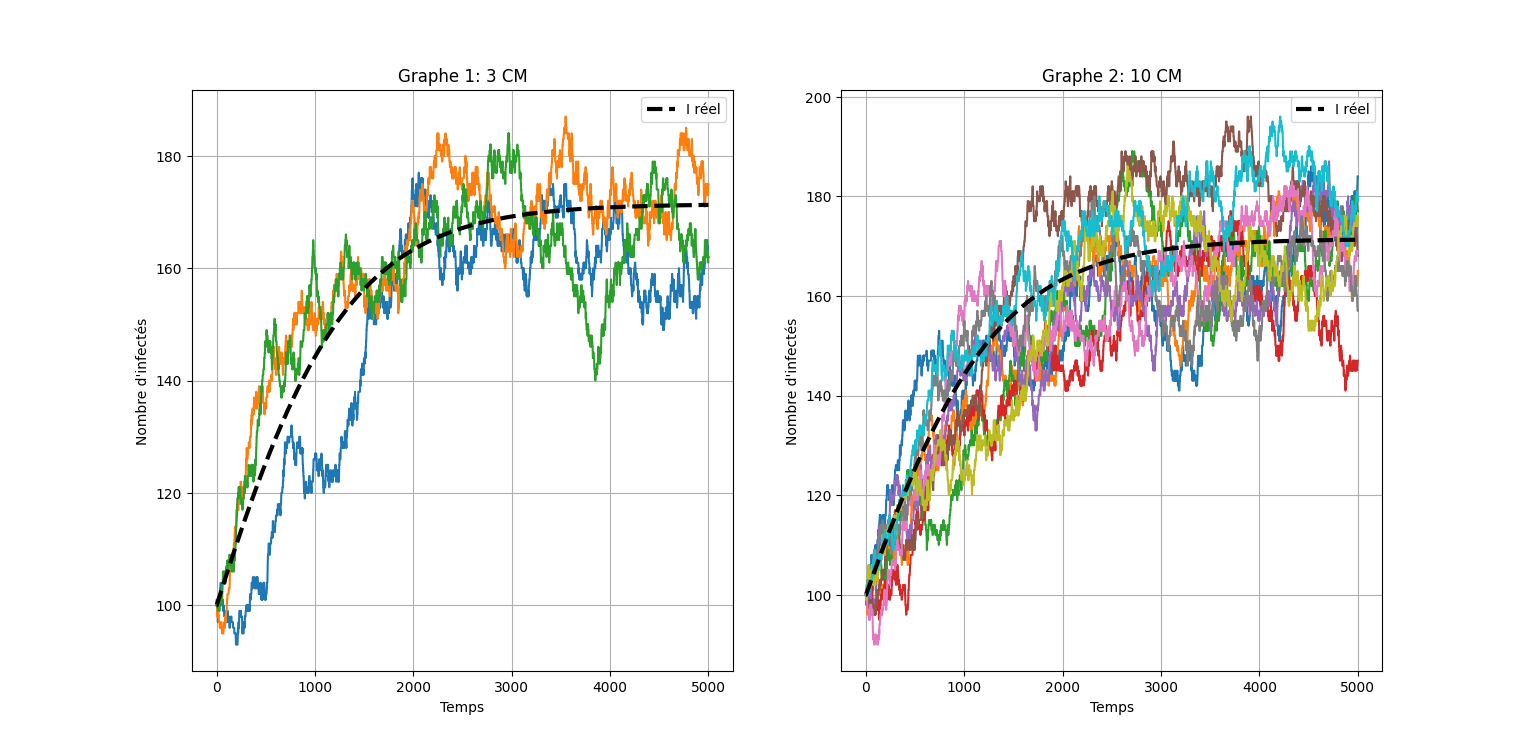
\includegraphics[width=0.75\textwidth]{im10-pr.png} % Ajustez le coefficient en fonction de vos besoins
  \caption{Évolution du nombre d'infectés}
  \label{fig:nb_inf2}
\end{figure}

Ces résultats peuvent être compris par loi forte. En effet, si on se donne une suite $(I^{N,r})_{r\in \mathbb{N}}$ de chaînes de Markov indépendantes et définies comme précédemment, pour le même jeu de paramètres $N, p, q$ avec la condition initiale déterministe $I^{N,r}_{0}=k$, on a par loi forte :
$$\forall t\in \mathbb{N}^*, \ \frac{1}{s} \sum_{r=1}^s I^{N,r}_t \xrightarrow[s \to \infty]{\text{p.s.}} \mathbb{E}(I^{N,1}_t)$$

Les simulations précédentes suggèrent que l'espérance précédente se rapproche de $N I_N(t)$. Un développement limité montre que c'est le cas pour $t=1$. Plus précisément, on peut montrer par un calcul qu'on a :
$$\mathbb{E} \left( \frac{1}{N}I^{N,1}_1 \right)-I_N(1) = o \left(\frac{1}{N} \right)$$

Si on veut plutôt faire le lien en temps continus, il suffit d'inverser l'échelle de temps. On simule des chaînes $I^N$ et on trace cette fois-ci les graphes de la chaîne de Markov et de la solution déterministe en temps continus. Plus précisément, on trace pour $t \in [0,1]$ la courbe de $I_N(t)$ ainsi que celle de $\frac{1}{N} I^N_{\lfloor Nt \rfloor}$. On choisit par exemple $N=100$ personnes dont $k=40$ personnes infectées initialement, $p=0,7$ et $q=0,3$ (figure~\ref{fig:taux_inf_lien}). \\

\begin{figure}[h!]
  \centering
  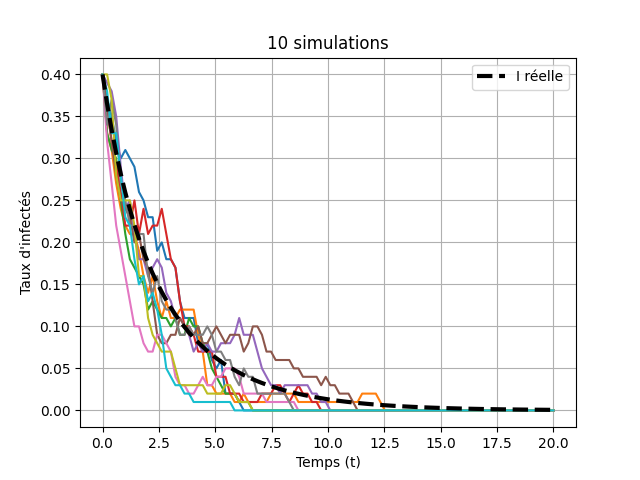
\includegraphics[width=0.45\textwidth]{im9-pr.png} % Ajustez le coefficient en fonction de vos besoins
  \caption{Evolution du taux d'infectés}
  \label{fig:taux_inf_lien}
\end{figure}

Notons que les fluctuations diminuent avec le nombre d'infectés $N$. Cela s'explique par théorème central limite. On le vérifie expérimentalement en regardant comment évolue la largeur de l'enveloppe convexe de $10$ courbes modélisant les nombres d'infectés en fonction du nombre d'individus dans la population pour un jeu de paramètres donné. Plus précisément, en fixant $\tau$ assez grand et en notant $(I^i_t)_{t \in \mathbb{N}}$, $i \in [1,10]$ dix réalisations de l'évolution du nombre d'infectés, on trace $\sup_{i,j \in [1,10], t \in [0,\tau]} |I^i(t)-I^j(t)|$ en fonction de $N$ (figure~\ref{fig:env_conv}). 

\begin{figure}[h!]
  \centering
  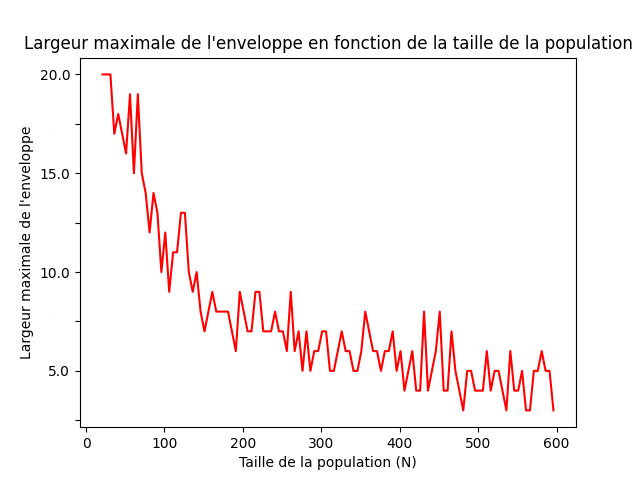
\includegraphics[width=0.45\textwidth]{im25-pr.png} % Ajustez le coefficient en fonction de vos besoins
  \caption{Enveloppe convexe des simulations en fonction du nombre d'individus dans la population}
  \label{fig:env_conv}
\end{figure}

On observe une décroissance en $\frac{1}{\sqrt{N}}$, comme prédit par le théorème central limite. \\

Pour finir, illustrons que lorsque $\R >1$, l'approximation du modèle déterministe par le modèle stochastique a ses limites. En effet, le nombre d'infectés revient à $0$ avec probabilité non nulle et cet état est absorbant. Si bien qu'en temps très long, le nombre d'infectés doit tomber à $0$, ce qui n'est pas le cas de la courbe déterministe. C'est ce qu'illustrent les figures suivantes (figure~\ref{fig:nb_inf_court}, figure~\ref{fig:nb_inf_moyen_terme} et figure~\ref{fig:nb_inf_long}) qui montrent des simulations du nombre d'infectés pour le même choix de paramètres mais sur diverses échelles de temps.

\begin{figure}[h!]
  \centering
  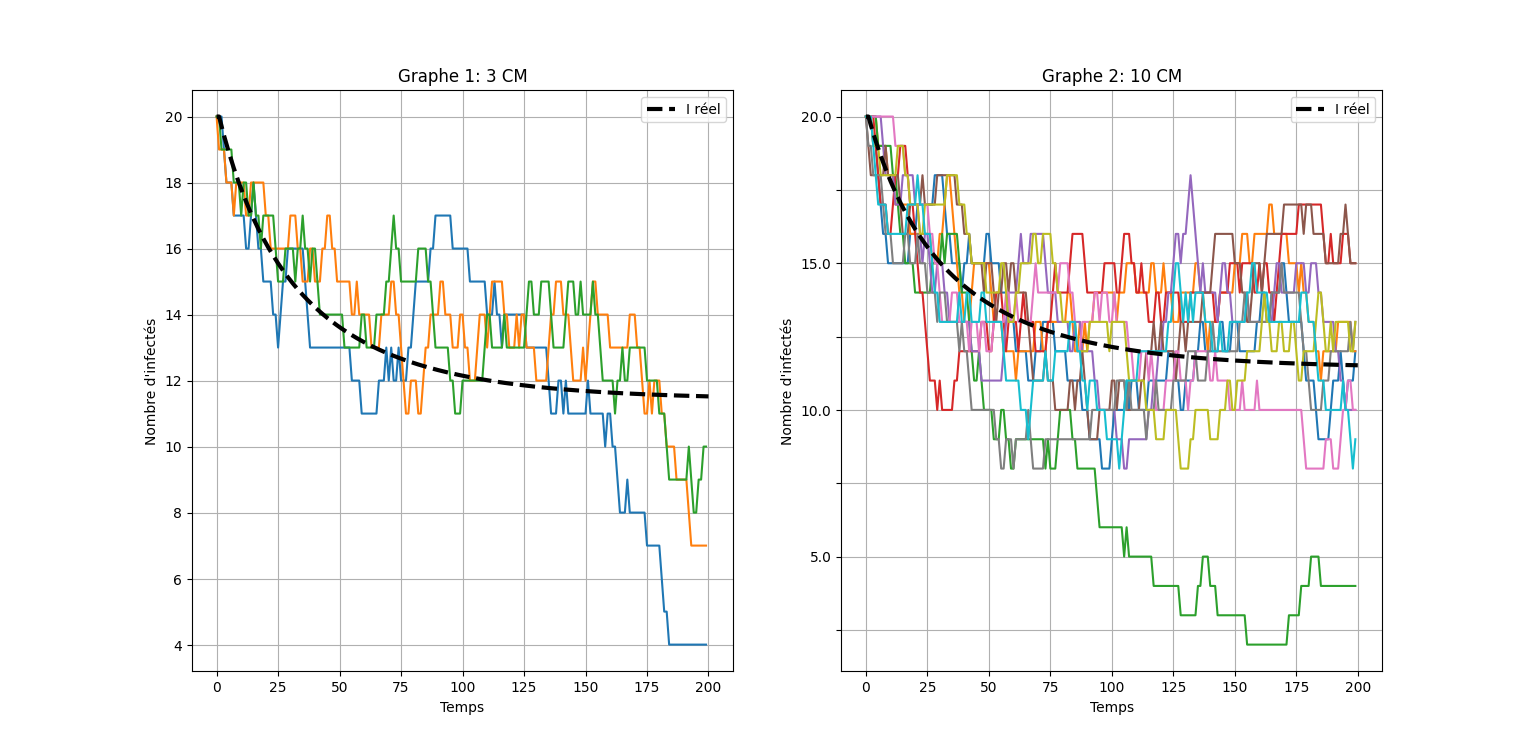
\includegraphics[width=0.7\textwidth]{im18-pr.png} % Ajustez le coefficient en fonction de vos besoins
  \caption{Evolution du nombre d'infectés en temps court}
  \label{fig:nb_inf_court}
\end{figure}


\begin{figure}[h!]
  \centering
  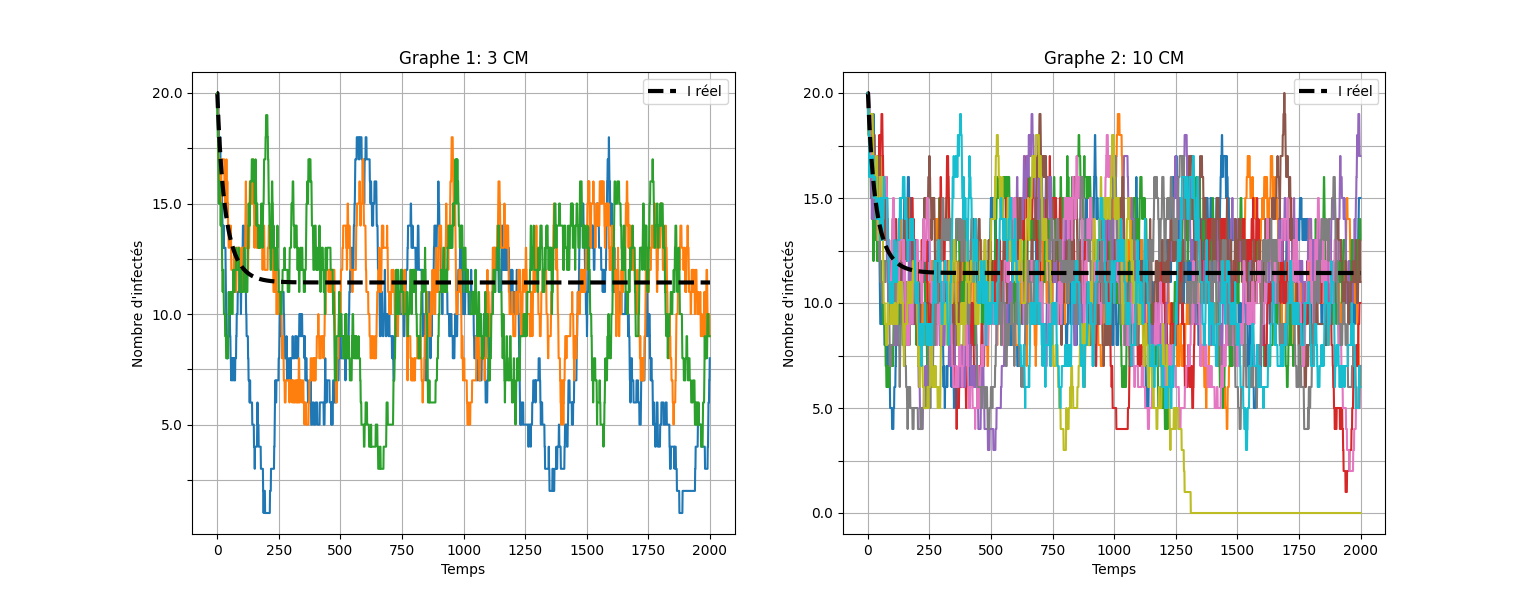
\includegraphics[width=0.7\textwidth]{im19-pr.png} % Ajustez le coefficient en fonction de vos besoins
  \caption{Evolution du nombre d'infectés à moyen terme}
  \label{fig:nb_inf_moyen_terme}
\end{figure}

\begin{figure}[h!]
  \centering
  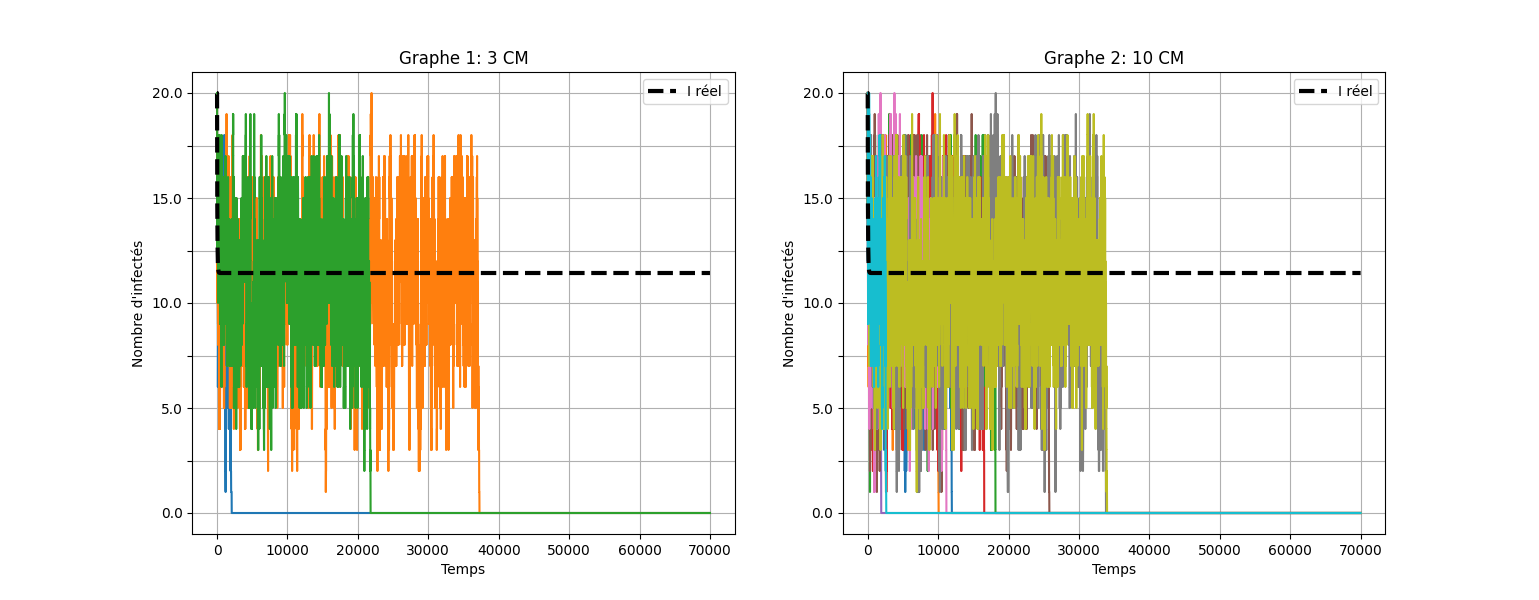
\includegraphics[width=0.7\textwidth]{im20-pr.png} % Ajustez le coefficient en fonction de vos besoins
  \caption{Evolution du nombre d'infectés en temps long}
  \label{fig:nb_inf_long}
\end{figure}
À court terme, les courbes des nombres d'infectés issues des simulations des processus stochastiques coïncident bien avec la courbe déterministe. À moyen terme, elles coïncident encore en moyenne avec la courbe déterministe. À long terme, on observe que les courbes des infectés issues des simulations tombent toutes à $0$ l'une après l'autre et ces chutes sont brutales.

\section{Modèle à plusieurs compartiments}

\subsection{Étude qualitative du modèle}
On souhaite à présent intégrer dans notre modèle la possibilité de déménager. On utilise à cet effet le processus suivant. \\

On prend un individu au hasard dans la population. En notant $i \in [0,n-1]$ l'indice de sa ville : \\
-- Avec probabilité $x$, on regarde sa position. S'il est sain, il déménage dans la ville $j\neq i$ avec probabilité $\frac{\varepsilon_{S}}{n-1} \alpha_{ij}$ où $(\alpha_{ij})_{ij}$ vérifie $\sum_{j \neq i} \alpha_{ij} = n-1$ quel que soit $i$ ; et reste dans la ville $i$ avec probabilité $1-\varepsilon_S$. S'il est infecté, c'est la même chose à ceci près que le coefficient $\varepsilon_S$ est remplacé par un coefficient $\varepsilon_I$.

-- Avec probabilité $1-x$, on regarde son état. S'il est malade, il guérit avec probabilité $p_i$. S'il est sain, on choisit un autre individu dans la même ville. Si cet autre individu est malade, il contamine le premier individu avec probabilité $q_i$ et s'il est sain, il ne se passe rien. \\

\subsection{Construction du modèle stochastique}

Pour la construction formelle, on se donne diverses suites de variables aléatoires : \\
-- Soit $(X_t)_{t \in \mathbb{N}^*}$ une suite de VAIID suivant la loi uniforme $\mathcal{U}([1,N])$. \\
-- Pour $i \in [0,n-1]$, soit $(R^{S,i}_t)_{t \in \mathbb{N}^*}$ une suite de VAIID telles que $\prob(R^{S,i}_t=0)=1- \varepsilon_S$ et pour $j \in [1,n-1]$, $\prob(R^{S,i}_t=j)=\frac{\varepsilon_S}{n-1} \alpha_{i,i+j}$. On définit également  $(R^I_t)_{t \in \mathbb{N}^*}$ une suite de VAIID ayant les mêmes propriétés, à ceci près qu'on remplace le coefficient $\varepsilon_S$ par le coefficient $\varepsilon_I$. \\
-- Pour toute partie $F \subset [1,N]$ non vide, soit $(X^F_{t})_{t \in \mathbb{N}^*}$ une suite de VAIID suivant la loi uniforme $\mathcal{U}(F)$. \\
-- Soit $(B_t)_{t \in \mathbb{N}^*}$ une suite de VAIID suivant la loi de Bernoulli $\mathcal{B}(x)$. \\
-- Pour $i \in [0,n-1]$, soit $(B^i_{1,t})_{t \in \mathbb{N}^*}$ une suite de VAIID suivant la loi de Bernoulli $\mathcal{B}(p_i)$ et $(B^i_{2,t})_{t \in \mathbb{N}^*}$ une suite de VAIID suivant la loi de Bernoulli $\mathcal{B}(q_i)$. \\

On suppose que toutes les suites de variables aléatoires introduites sont indépendantes. \\

On cherche à définir $M^N$, matrice aléatoire de taille $2 \times N$ de telle sorte que pour $k \in [1,N]$, $M^N_{t,(1,k)}$ soit égal à $1$ si l'individu $k$ est infecté et $0$ sinon ; et $M^N_{t,(2,k)}$ est le numéro de la ville de l'individu $k$. On définit les numéros de ville modulo $n$ pour simplifier. \\ 

On se donne à cet effet $M^N_0$ matrice de taille $2 \times N$ déterministe. Dans la suite, on notera $(n_i)$ et $(k_i)$ respectivement les nombres de personnes et d'infectés initiaux de chaque groupe. On définit alors :
$$M^{N}_{t+1}=f(M^N_{t+1},X_{t+1},(R^{I,i}_{t+1})_i,(R^{S,i}_{t+1})_i,(X^F_{t+1})_F,B_{t+1},(B^i_{1,t+1})_{i \in [0,n-1]},(B^i_{2,t+1})_{i \in [0,n-1]})$$
où $f$ est la fonction mesurable qui permet de modéliser le processus décrit en introduction. \\

Plus précisément : \\

$f(M,k,(r^{I,i})_i,(r^{S,i})_i,(k_F)_{F},m,(m^i_1)_{i}, (m^i_2)_{i}) =
\left\{
\begin{array}{ll}
    M + rE_{2,k} & \text{si } m = 1 \\
    M - m^{i_0}_{1} E_{1,k} & \text{si } M_{1,k} = 1 \text{ et } m = 0 \\
    M + m^{i_0}_{2}E_{1,k} & \text{si } M_{1,k_{F(i_0)}} = 1, M_{1,k} = 0 \text{ et } m = 0 \\
    M & \text{si } M_{1,k_{F(i_0)}} = 0, M_{1,k} = 0 \text{ et } m = 0
\end{array}
\right.$\\
où $i_0=M_{2,k}$ est la ville de l'individu $k$, $F(i_0)$ est l'ensemble des personnes dans la ville $i_0$ et $r=r^{I,i_0}$ si $k$ est infecté i.e. $M_{1,k}=1$ et $r^{S,i0}$ sinon. \\

Pour $x=1$, on retrouve un modèle de marche aléatoire et pour $x=0$ on observe $n$ villes isolées, voir (figure~\ref{fig:nb_inf_x}).

\begin{figure}[h]
    \centering
    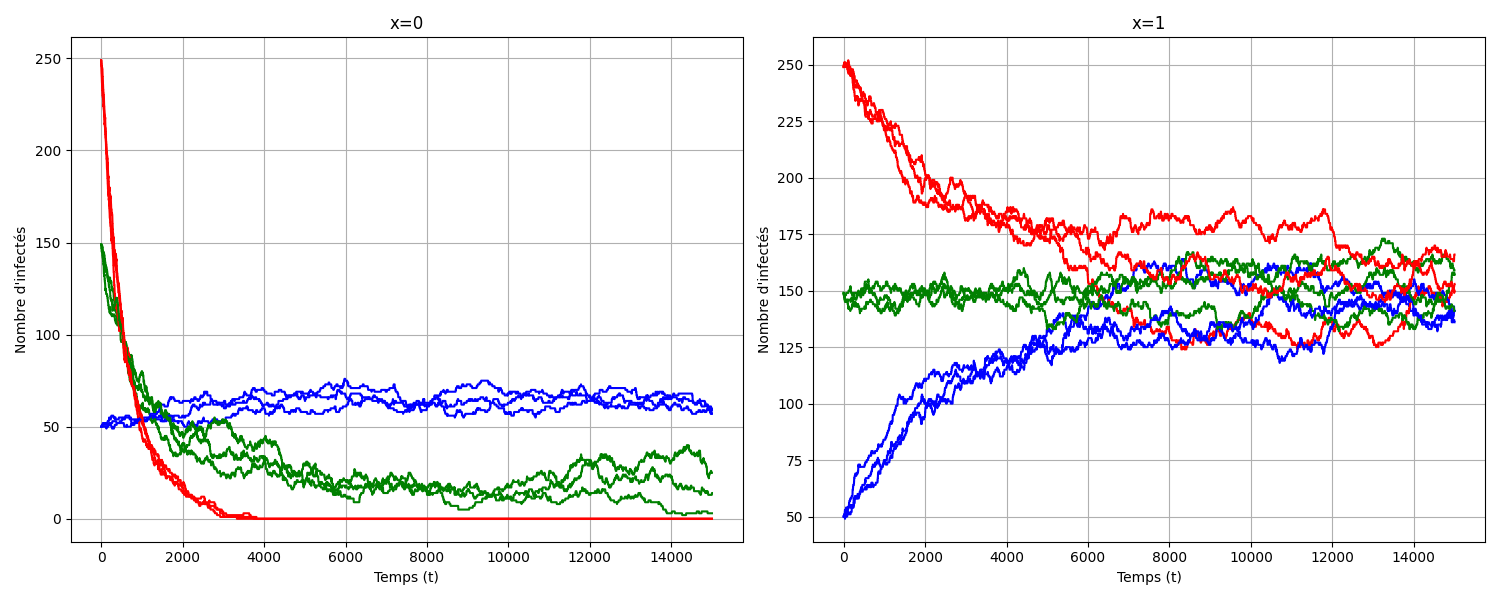
\includegraphics[width=0.65\textwidth]{im24-pr.png}
    \caption{Évolution du nombre d'infectés pour $x=0$ et $x=1$}
    \label{fig:nb_inf_x}
\end{figure}

Dans le cas $x=1$, on retrouve bien qu'en temps long le nombre d'infectés des différente villes s'homogénéise. On est donc bien le cadre de la section $2$. Dans le cas $x=0$, les infectés des différentes villes évoluent de façon indépendante.

\subsection{Construction du modèle déterministe associé}

On cherche à construire un modèle déterministe à partir du modèle stochastique précédent. On veut trouver une équation différentielle en se basant sur l'intuition suivante :
$$\mathbb{E}(I^{N,i}_1) = I_i(\Delta_N) \simeq I_i(0)+\Delta_N I'_i(0)$$
Plus précisément, on approxime le nombre d'infectés du groupe $i$ du modèle stochastique à l'instant $t=1$ par le nombre d'infectés du modèle stochastique à l'instant $\Delta_N$ en grandes populations.

On peut montrer que :
$$\E(I^{N,i}_1)=k_i+\frac{1}{N} \left( d_I^0 \sum_{j \in \Omega} L_{i,j} k_j + \beta_i^0 \frac{(n_i-k_i) k_i}{n_i}-\gamma_i^0 k_i \right)$$
avec $L_{i,j}=\alpha_{ij}/(n-1)$ si $i \neq j$ et $-1$ si $i=j$; $\gamma_i^0=(1-x)p_i$; $\beta_i^0=(1-x)q_i$; $d_I^0=x\varepsilon_I$. \\

On choisit plutôt le pas de temps $\Delta_N = \frac{1}{Na}$ ; où $a >0$ afin de se laisser un paramètre libre $a$ que l'on pourra adapter au besoin. On écrit donc :
$$\E(I^{N,i}_1)=k_i+\frac{1}{Na} \left( ad_I^0 \sum_{j \in \Omega} L_{i,j} k_j + a\beta_i^0 \frac{(n_i-k_i) k_i}{n_i}-a\gamma_i^0 k_i \right)$$

De même, on peut montrer que  :
$$\E(S^{N,i}_1)=k_i+\frac{1}{N} \left(d_S^0 \sum_{j \in \Omega} L_{i,j} ( n_j-k_j) - \beta_i^0 \frac{(n_i-k_i) k_i}{n_i}+\gamma_i^0 k_i \right)$$
où $d_S^0 = x\varepsilon_S$. \\

\begin{tabular}{|c}
\begin{minipage}{\textwidth}
Le système d'équations différentielles déterministes à étudier est donc le suivant :
\[
\left\{
\begin{aligned}
\frac{dI_i}{dt} &= d_I \sum_{j \in \Omega} L_{i,j} I_j + \beta_i\frac{S_i I_i}{S_i+I_i} - \gamma_i I_i \\
\frac{dS_i}{dt} &= d_S \sum_{j \in \Omega} L_{i,j} S_j - \beta_i\frac{S_i I_i}{S_i+I_i} + \gamma_i I_i
\end{aligned}
\right.
\]
pour $i \in \Omega = [0,n-1]$, où $d_I=ad_I^0$, $d_S=a d_S^0$, $\gamma_i=a\gamma_i^0$ et $\beta_i=a\beta_i^0$.
\end{minipage}
\end{tabular} \\

\subsection{Convergence du modèle stochastique vers le modèle déterministe : simulations}
On résout numériquement ce système d'équations différentielles en Python et on simule plusieurs fois la population avec le processus stochastique. Via le changement d'échelle de temps continu/discret $t_{\text{discret}}=\lfloor Nat \rfloor$, on peut superposer les courbes des infectés simulées par le modèle stochastique et les courbes données par la résolution du système d'équations différentielles déterministes (figure~\ref{fig:nb_inf_syst_ed}). Cela illustre la convergence du modèle stochastique vers le modèle déterministe.

\begin{figure}[h]
    \centering
    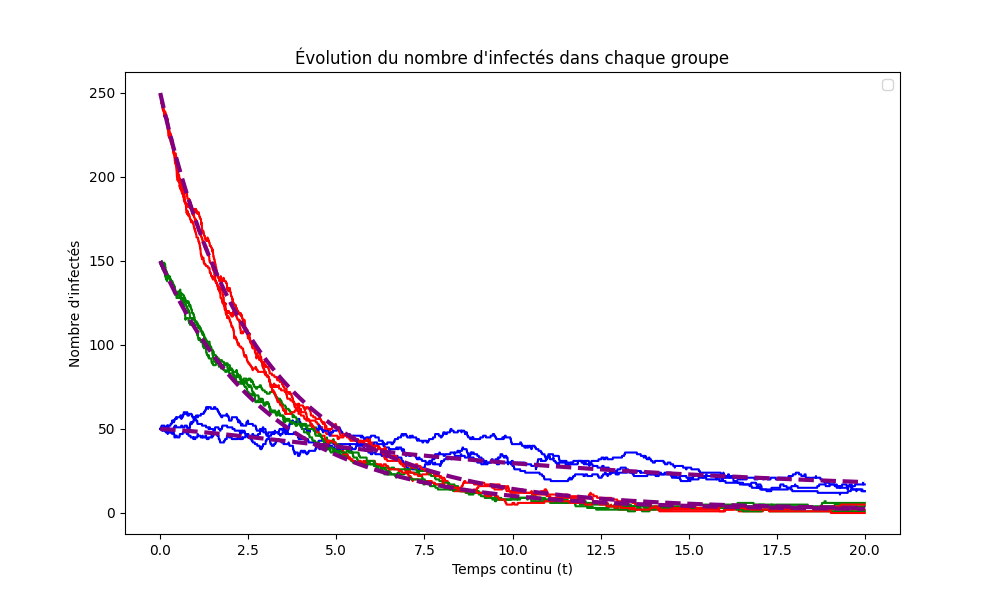
\includegraphics[width=0.7\textwidth]{im23-pr.png}
    \caption{Évolution du nombre d'infectés}
    \label{fig:nb_inf_syst_ed}
\end{figure}

La figure~\ref{fig:nb_inf_syst_ed} est donnée pour $N=500$ individus répartis dans $n=3$ villes, avec un jeu de coefficients $(p_i),(q_i)$ quelconque, $\varepsilon_S=\varepsilon_I=0,1$ et $x=0,5$. \\

On remarque que : \\
-- $L$ est \textbf{irréductible}, c'est-à-dire que pour $i\neq j$, il existe $p \in \mathbb{N}^*$ tel que $[L^p]_{i,j}\neq 0$, et symétrique. \\
-- $L$ est \textbf{essentiellement positive} i.e. pour $i \neq j$, $L_{i,j}>0$. \\

On fait de plus les hypothèses suivantes : \\
-- Les $p_i$ sont non nuls. \\ 
-- En notant $\R^{(i)}=\frac{q_i}{p_i}$, il existe $i,j \in [0,n-1]$ tels que $\R^{(i)}>1$, $\R^{(j)}<1$ et pour tout $k \in [0,n-1]$, $\R^{(k)}\neq 1$. \\

Ces hypothèses vont nous permettre de bénéficier des résultats donnés dans \cite{GaoDong}.  \\

On pose $F=\text{Diag}(\beta_0,...,\beta_{n-1})$ et $V=\text{Diag}(\gamma_0,...,\gamma_{n-1})-d_I L$.

Par \textbf{théorème de Gerschgorin} (voir \cite{Gerschgorin}), en notant $B(x,r)$ la boule centrée en $x$ et de rayon $r$ pour la norme euclidienne : 
$$\text{Sp}(V) \subset \cup_{i=1}^n B(\gamma_i-d_I L_{ii}, d_I |L_{ii}|)$$
Comme pour tout $i$, $\gamma_i > 0$, $L_{ii}\leq 0$ et $d_I\geq 0$, ces boules ne contiennent pas $0$ et par conséquent $0$ n'est pas valeur propre de $V$ i.e. $V$ est inversible. \\

On peut alors définir alors le nombre de reproduction de base $\R$ par :
$$\boxed{\R=\rho(F V^{-1})}$$

Lorsqu'il n'y a pas de coefficients de diffusion ($d_I=d_S=0$), les équations pour chaque groupe sont indépendantes des équations pour les autres groupes, si bien qu'on est ramené à étudier le système :
\[
\left\{
\begin{aligned}
\frac{dI}{dt} &= \beta\frac{SI}{S+I} - \gamma I \\
\frac{dS}{dt} &= - \beta\frac{S I}{S+I} + \gamma I
\end{aligned}
\right.
\]
On retrouve les équations du modèle SIS. En sommant ces deux équations, on obtient également que $I+S=N$ est une constante. 

On vérifie aisément que le $\R$ du modèle SIS et le $\R$ donné pour le modèle à plusieurs compartiments coïncident dans ce cas particulier.
\subsection{Propriétés du $\R$}

On s'intéresse à présent aux propriétés du $\R$. On a le résultat suivant issu de \cite{GaoDong} : \\

\begin{tabular}{|c}
\begin{minipage}{\textwidth}
\textbf{Proposition} \\
La fonction $d_I \mapsto \R (d_I)$ est strictement décroissante et strictement convexe sur $]0,+ \infty[$.
\end{minipage}
\end{tabular} \\ 
 
\begin{proof}
On peut obtenir ce résultat en s'intéressant aux variations du rayon spectral vu comme fonction de $d_I$. Le rayon spectral défini sur les matrices symétriques est suffisamment lisse en dehors de $0$ car il coïncide avec la norme subordonnée à la norme $2$ sur les matrices normales (i.e. qui commutent avec leur transposée). \\

Des compléments sur la régularité du rayon spectral peuvent être trouvés dans \cite{Kloeckner2019}.
\end{proof}

Comme $d_I$ est fonction croissante de $\varepsilon_I$, on en déduit que le $\R$ diminue avec $\varepsilon_I$. Il est donc préférable de laisser les individus déménager afin de diminuer le $\R$.

On peut tracer le graphe de $\R$ en fonction de $\varepsilon_I$ pour différentes valeurs de $x$ (figure~\ref{fig:evol_r0}).

\begin{figure}[h]
    \centering
    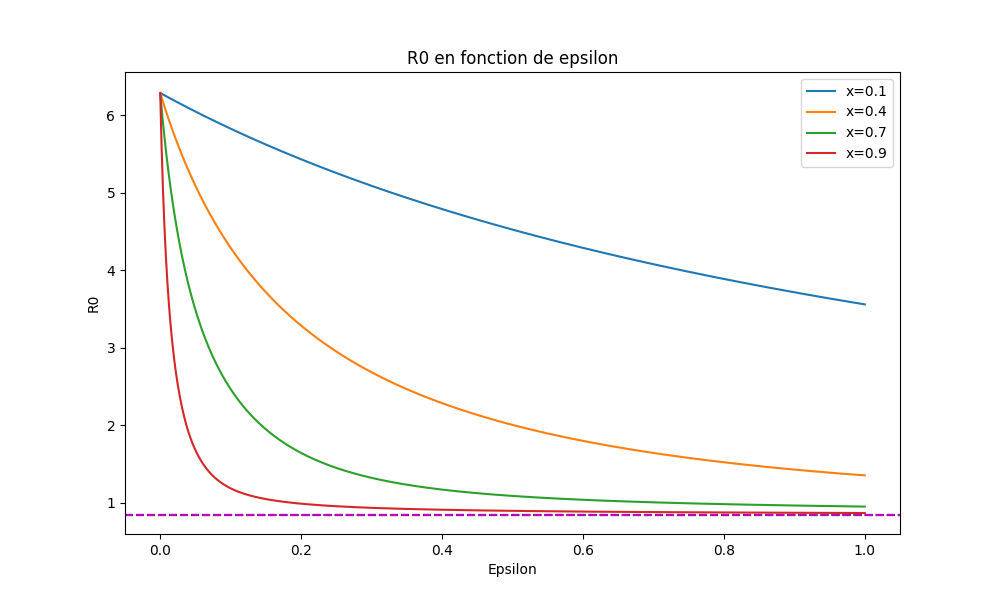
\includegraphics[width=0.7\textwidth]{im22-pr.png}
    \caption{Graphe de $\varepsilon \mapsto \R$ pour divers $x$}
    \label{fig:evol_r0}
\end{figure}

On constate que plus la probabilité d'effectuer une action de déplacement $x$ est proche de $1$, plus le $\R$ diminue et plus il diminue vite avec $\varepsilon$. \\

On a par ailleurs l'encadrement suivant issu de \cite{GaoDong}. : \\

\begin{tabular}{|c}
\begin{minipage}{\textwidth}
\textbf{Proposition} \\
$\R$ vérifie :
$$\boxed{\min_{i \in [0,n-1]} \R^{(i)} < \R(\infty)=\frac{\sum_{i \in \Omega} \gamma_i L^*_{ii}}{\sum_{i \in \Omega} \beta_i L^*_{ii}} <  \R(0)=\max_{i \in [0,n-1]} \R^{(i)}}$$
où $L^*$ est la transposée de la comatrice de $L$ et $\R(\infty)$ est la limite de $\R$ lorsque $d_I \longrightarrow + \infty$.
\end{minipage}
\end{tabular} \\

On note que la limite en $+ \infty$ précédente existe car $\R$ est décroissante et minorée par 0. De plus, elle ne dépend pas de $x$ car  $\gamma_i=a(1-x)p_i$ et $\beta_i=a(1-x)q_i$ donc il y a simplification dans le quotient ci-dessus. La limite $\R(\infty)$ en l'infini de la fonction $d_I \mapsto \R (d_I)$ est tracée en pointillés dans le graphe de de la figure~\ref{fig:evol_r0}. \\

L'égalité $\R(0)=\max_{i \in [0,n-1]} \R^{(i)}$ traduit le fait que si on empêche les déménagements des personnes infectées (i.e. $\varepsilon_I=0$), alors le nombre de reproduction de base est le maximum des nombres de reproduction de base locaux des différentes villes. \\

On note $\sum_{\beta}=(-1)^{n-1} \sum_{i \in \Omega} \beta_i L^*_{ii}$ et $\sum_{\gamma}=(-1)^{n-1} \sum_{i \in \Omega} \gamma_i L^*_{ii}$. On dit qu'on est dans un domaine : \\
-- à \textbf{bas risque} si $\sum_{\beta} < \sum_{\gamma}$. \\
-- à \textbf{haut risque} si $\sum_{\beta} \geq \sum_{\gamma}$. \\

En remarquant que $(-1)^{n-1}(L_{11}^*,...,L_{nn}^*)>0$ par  corollaire 6.2.27 dans Horn et Johnson \cite{HornJohnson}, on a le résultat suivant comme conséquence des résultats précédents : \\

\begin{tabular}{|c}
\begin{minipage}{\textwidth}
\textbf{Proposition} \\
Si $\R(0) = \text{max}_{i \in  \Omega} \R^{(i)} > 1$. Alors : \\

\textbf{1/} Dans un domaine à bas risque, il existe un unique seuil $d_I^* \in ]0, + \infty[$ vérifiant $\det(F-V)=\det(F-D+d_I^* L)=0$ tel que $\R(d_I)>1$ pour $d_I<d_I^*$ et $\R(d_I)<1$ pour $d_I>d_I^*$. \\

\textbf{2/} Dans un domaine à haut risque, $\R(d_I) > 1$ pour tout $d_I \geq 0$.

\end{minipage}
\end{tabular} \\

\subsection{Équilibre endémique}
On introduit dans cette section la notion d'équilibre endémique. Intuitivement, le concept d'équilibre endémique en épidémiologie mathématique représente un état stable de l'épidémie. \\

Mathématiquement, on dit que $E^*=(S^*, I^*)=(S_1^*,...,S_n^*, I_1^*,...,I_n^*)$ est un \textbf{équilibre endémique} si $E^*$ vérifie le système : \\
$$\left\{
\begin{aligned}
& d_S\sum_{j \in \Omega} L_{ij}S_j^* - \beta_i \frac{S_i^* I_i^*}{S_i^* + I_i^*} + \gamma_i I_i^* = 0 \\
& d_I \sum_{j \in \Omega} L_{ij} I_j^* + \beta_i \frac{S_i^* I_i^*}{S_i^*+I_i^*} - \gamma_i I_i^* = 0
\end{aligned}
\right.$$ \\

On trouve dans \cite{Allen2007} le résultat suivant : \\

\begin{tabular}{|c}
\begin{minipage}{\textwidth}
\textbf{Proposition} \\
Si $\R > 1$, le modèle admet un unique équilibre endémique. Si $\R < 1$, le modèle est globalement asymptotiquement stable : il n'y a pas d'équilibre endémique.
\end{minipage}
\end{tabular} \\

Ce résultat traduit le fait que le $\R$ joue bien son rôle i.e. il permet de prévoir l'évolution de l'épidémie. \\

En vertu de ce résultat, lorsque $\R (\infty) > 1$ (et que par décroissance de $\R$, pour tout $d_I\geq 0$, $\R(d_I) > 1$), on peut définir la fonction $d_I \mapsto E^*(d_I)$ qui au coefficient de diffusion $d_I$ associe l'unique équilibre endémique. On a de plus le résultat suivant, donné dans \cite{GaoDong} : \\

\begin{tabular}{|c}
\begin{minipage}{\textwidth}
\textbf{Proposition} \\
Si $\R(\infty) > 1$, alors :
$$E^*(d_I) \underset{d_I \to +\infty}{\longrightarrow} m \times (\hat{S_1},...,\hat{S_n},|L_{11}^*|,...,|L_{nn}^*|)$$
où $(\hat{S_1},...,\hat{S_n})$ est l'unique solution $>0$ de :
$$d_S \sum_{j \in \Omega} L_{ij} \hat{S_j} - \beta_i \frac{|L_{ii}^*|}{\hat{S_i} + |L_{ii}^*|} \hat{S_i} + \gamma_i |L_{ii}^*| = 0$$
et :
$$m=\frac{\sum_{i=1}^n (S_i(0)+I_i(0))}{\sum_{i=1}^n (\hat{S_i} + |L_{ii}^*|)}$$
\end{minipage}
\end{tabular} \\

Illustrons graphiquement la validité de ce résultat. On résout numériquement le système d'équations différentielles pour des valeurs de $d_I \longrightarrow + \infty$ et on observe l'équilibre vers lequel tend le nombre d'infectés dans un groupe choisi (que l'on note $i$) est bien celui donné par le résultat précédent. Voir figure~\ref{fig:nb_inf_di}. \\

\begin{figure}[h!]
  \centering
  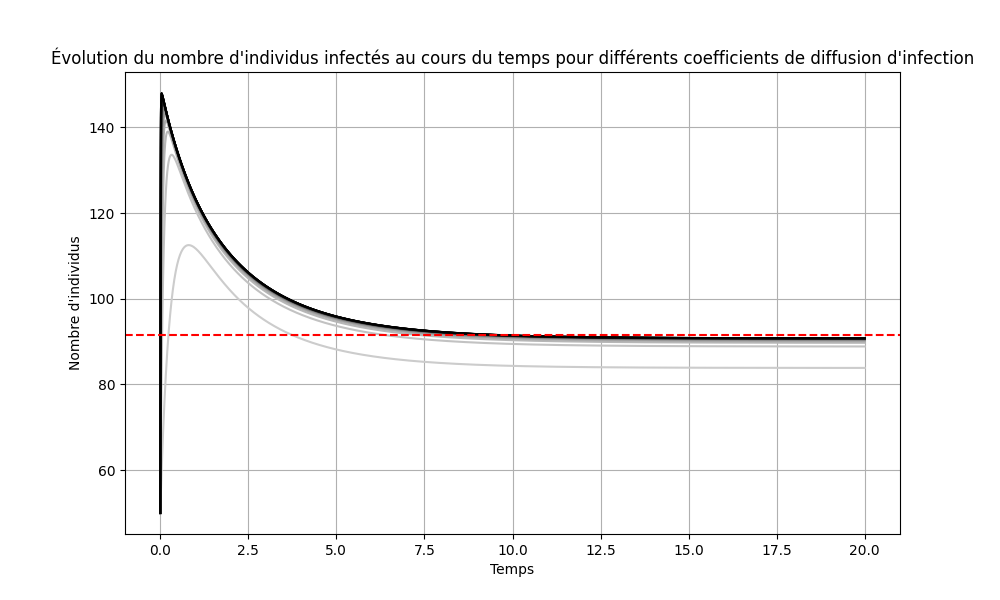
\includegraphics[width=0.6\textwidth]{im26-pr.png} % Ajustez le coefficient en fonction de vos besoins
  \caption{Évolution du nombre d'infectés selon pour des valeurs $d_I$ de plus en plus grandes}
  \label{fig:nb_inf_di}
\end{figure}

La droite rouge est la droite d'équation $y=m \times |L_{ii}^*|$. \\

\subsection{Répartition des individus dans les villes}

On s'intéresse dans cette section à la répartition des individus dans les groupes, sans tenir compte de leur nature (infecté ou susceptible). Pour cela, on somme les deux équations du système d'équations différentielles modélisant l'épidémie. On obtient, en notant $N_i$ le nombre de personnes dans le groupe $i$ :
$$\frac{d N_i}{dt} = (d_S+d_I) \sum_{j=1}^n L_{ij} N_j$$ 
Ce que l'on écrit sous forme matricielle :
$$\boxed{\frac{dN}{dt} = AN}$$
où $A=(d_I+d_S)L$. \\
On a donc $N(t)=P_t N_0$ où $P_t=e^{tA}$ et $N_0$ est la répartition initiale des individus dans les différents groupes. \\

Le résultat suivant donne des propriétés vérifiées par $P_t$ : \\

\begin{tabular}{|c}
\begin{minipage}{\textwidth}
\textbf{Proposition} \\
-- $\forall t \geq 0, \ \ P_t \textbf{1} = \textbf{1}$ \\
-- $\forall s, t \geq 0, \ \ P_{s+t} = P_s P_t$ \\
-- $\forall t \geq 0$, $P_t \geq 0$
\end{minipage}
\end{tabular} 

\begin{proof}
Le premier point vient du fait que $A \textbf{1} = \textbf{0}$ car la somme des colonnes de $L$ est nulle. Le deuxième point est immédiat. Pour le troisième point, on écrit :
$$P_t \underset{t \rightarrow 0}{=} I + t(d_I=d_S)L + o(t)$$
Comme $L$ est essentiellement positive, on en déduit qu'il existe $\varepsilon > 0$ tel que pour tout $t \in [0, \varepsilon], P_t \geq 0$. Ainsi, pour $t \geq 0$ quelconque, on écrit $t=n \varepsilon + r$ où $n \in \mathbb{N}$ et $0 \leq r < \varepsilon$. Si bien qu'en utilisant le deuxième point et ce qui précède :
$$P_t = (P_{\varepsilon})^n P_r \geq 0$$
Ce qui conclut.
\end{proof}

On a finalement le résultat de répartition de population suivant : \\

\begin{tabular}{|c}
\begin{minipage}{\textwidth}
\textbf{Proposition} \\
En temps long, la population s'équilibre dans les différents groupes.
\end{minipage}
\end{tabular}

\begin{proof}
Par \textbf{théorème de Gerschgorin} \cite{Gerschgorin}, on a :
$$\text{Sp}(A) \subset \cup_{i=1}^n B((d_I+d_S)L_{ii}, (d_I+d_S)|L_{ii}|)$$
Ces disques contiennent uniquement des réels négatifs, ce qui montre que les valeurs propres de $A$ sont négatives. \\

En notant $\lambda_1=0 > ... > \lambda_p$ les valeurs propres distinctes de $A$ et $\text{Proj}^{i}$ la projection sur l'espace propre $E_{\lambda_i}(A)$, on écrit :
\begin{align*}
N(t) & = e^{tA} N_0 \\
& = \left( \text{Proj}^{1} + \sum_{i \geq 2} e^{t \lambda_i} \text{Proj}^i \right)N_0
\end{align*}
et pour tout $i \geq 2$, $e^{t \lambda_i} \underset{t \to \infty}{\longrightarrow} 0$ car $\lambda_i < 0$.
Par suite :
$$\boxed{N(t) \underset{t \to \infty}{\longrightarrow} \text{Proj}^1 N_0 = \frac{(N_0, \textbf{1})}{(\textbf{1}, \textbf{1})} \textbf{1}}$$
en remarquant que $E_0(A)$ est engendré par $\textbf{1}$ car la valeur propre $1$ est simple par théorème de Perron-Frobenius \cite{Perron}.
\end{proof}

\section{Perspectives} 

Le résultat précédent nous incite à supposer, dans le cadre d'une étude d'équilibre, que $S_i+I_i$ ne dépend ni de $i$ ni de $t$. On note cette constante $C$. On pose alors $u_i(t)=I_i(t)/C$. Notre système d'équations différentielles s'écrit alors :
$$\partial_t u = F(u)$$
où $F(u) = d_I Lu + \beta (1-u) - \gamma u$. \\

Il semble qu'on est dans le cadre d'application des résultats de \cite{DronnierThesis}, chapitre II. On doit pouvoir montrer que $F$ est coopérative et localement lipschitzienne dans un cadre adapté. \\ 
On pourrait introduire le semi-flot $\phi$ : 
$$\left\{
\begin{aligned}
& \partial_t \phi(t,g) = F(\phi(t,g)) \\
& \phi(0,g)=g
\end{aligned}
\right.$$ 
On devrait pouvoir montrer, comme dans \cite{DronnierThesis}, des résultats du type :  \\

\begin{tabular}{|c}
\begin{minipage}{\textwidth}
\textbf{Proposition} \\
Si $0 \leq g \leq h \leq 1$, alors :
$$\forall t \geq 0, \ \ \phi(t, g) \leq \phi(t,h)$$
\end{minipage}
\end{tabular} \\

Ainsi que : \\

\begin{tabular}{|c}
\begin{minipage}{\textwidth}
\textbf{Proposition} \\
Le chemin $t \mapsto \phi(t,g)$ est croissant (resp. décroissant) si et seulement si $F(g) \geq 0$ (resp. $F(g) \leq 0$).
\end{minipage}
\end{tabular} \\

Ainsi, comme $F(\textbf{1}) = -\gamma \textbf{1} \leq 0$, on doit obtenir que les nombres d'infectés des différents groupes décroissent si on part de $100 \%$ d'infectés.

\section{Conclusion}

On est parti d'un modèle stochastique simple d'abord à un compartiment puis à plusieurs compartiments et on a étudié ses propriétés. Par un passage à la limite, on a trouvé un modèle déterministe à partir de ce modèle stochastique. On a vérifié expérimentalement que les deux modèles correspondaient. \\

On retient de ce projet les faits suivants : \\
-- Le $\R$ permet de prédire comment va évoluer l'épidémie. \\
-- Laisser les individus se déplacer permet de diminuer le $\R$ de l'épidémie et donc lorsque $\R < 1$ de faire disparaître la maladie. \\
-- On a réussi à lier notre modèle stochastique d'épidémie à un modèle déterministe, mais cela a ses limites lorsque $\R > 1$ car la maladie finit toujours par s'éteindre en temps très long dans le modèle stochastique mais pas dans le modèle déterministe. \\

\textbf{Remerciements.} Je tiens à remercier Jean-François Delmas, qui m'a suivi durant tout ce projet en me donnant
des ressources, des conseils et en prenant le temps de m'expliquer des points techniques précis.


\newpage

\bibliographystyle{IEEEtran}
\bibliography{biblio}{}



\end{document}